%%%% CAPÍTULO 2 - REVISÃO DA LITERATURA (OU REVISÃO BIBLIOGRÁFICA, ESTADO DA ARTE, ESTADO DO CONHECIMENTO)
%%
%% O autor deve registrar seu conhecimento sobre a
%% literatura básica do assunto, discutindo e 
%% comentando a informação já publicada. A revisão deve
%% ser apresentada, preferencialmente, em ordem
%% cronológica e por blocos de assunto, procurando
%% mostrar a evolução do tema.

%% Título e rótulo de capítulo (rótulos não devem conter caracteres especiais, acentuados ou cedilha)
\chapter{Estrutura e Mecânica}\label{cap:Mecânica}

Neste capítulo, abordaremos em detalhes a concepção e a implementação das partes mecânicas e estruturais do nosso projeto. A integração entre esses dois aspectos é fundamental para garantir a precisão e a eficiência do 3D Scan, razão pela qual os discutimos em conjunto em um mesmo capítulo.

A estrutura do mesmo foi inteiramente projetada e construída utilizando peças de impressão 3D, uma escolha que nos permitiu grande flexibilidade, customização e economia. Tendo também, a facilidade de ajustar e reconstruir a peça, se necessário.

A mecânica está intrinsecamente conectada à estrutura, composta por eixos e rolamentos que permitem movimentos suaves e precisos. Para garantir o controle exato desses movimentos, utilizamos motores de passo Nema17, que são essenciais para a operação sincronizada do 3D Scan e para a obtenção das distâncias dos pontos captados.

Neste capítulo, detalharemos o design estrutural e os materiais utilizados. Em seguida, exploraremos a configuração mecânica, discutindo a escolha dos componentes, sua integração na estrutura impressa e a metodologia adotada para garantir o alinhamento e a calibração necessários para um desempenho satisfatório do projeto.

\section{Componentes da estrutura}

%tabela dos componentes com o preço
%explicação breve sobre cada um deles

Para o desenvolvimento do projeto, foram necessárias as seguintes partes estruturais:

\begin{table}[h]%% Ambiente table
\caption{Componentes e Orçamento}%% Legenda
\label{table:items}%% Rótulo
\begin{tabularx}{\textwidth}{@{\extracolsep{\fill}}lc}%% Ambiente tabularx
\toprule
Descrição & Valor \\
\midrule
Acoplador do Eixo           & R\$9,00 \\
Fixador do Motor            & R\$9,00 \\
Bases dos Motores          & R\$72,00 \\
Plataforma do Sensor        & R\$35,00 \\
Mesa Giratória              & R\$35,00 \\
Guia Superior               & R\$15,00  \\
Eixos 8mm                   & R\$38,98  \\
Rolamentos 8mm              & R\$25,52  \\
\bottomrule
\end{tabularx}
\fonte{AUTORES}%% Fonte
\end{table}

A seguir podemos observar a modelagem 3D dos componentes (Figura 1) e sua estrutura final (Figura 2).

\begin{figure}[H]
\captionsetup{width=0.6\textwidth}%% Largura da legenda
\caption{Modelagem 3D}%% Legenda
\label{foto:eletronica_frontal}%% Rótulo
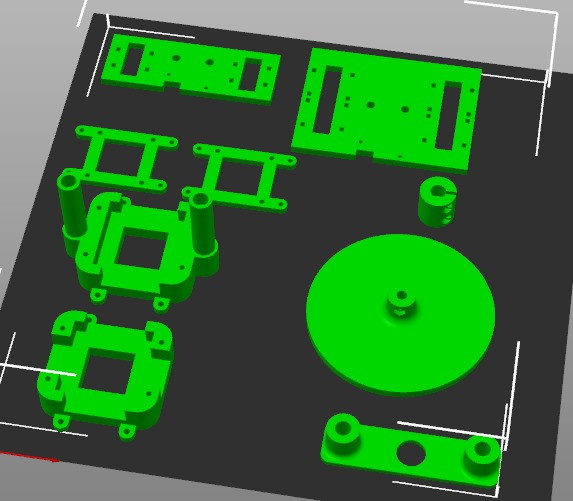
\includegraphics[width=0.45\textwidth]{3.Mecânica/Imagem/STL.jpeg}%% Dimensões e localização
\fonte{AUTORES}%% Fonte
\end{figure}

\begin{figure}[H]
\captionsetup{width=0.6\textwidth}%% Largura da legenda
\caption{Estrutura Final}%% Legenda
\label{foto:eletronica_frontal}%% Rótulo
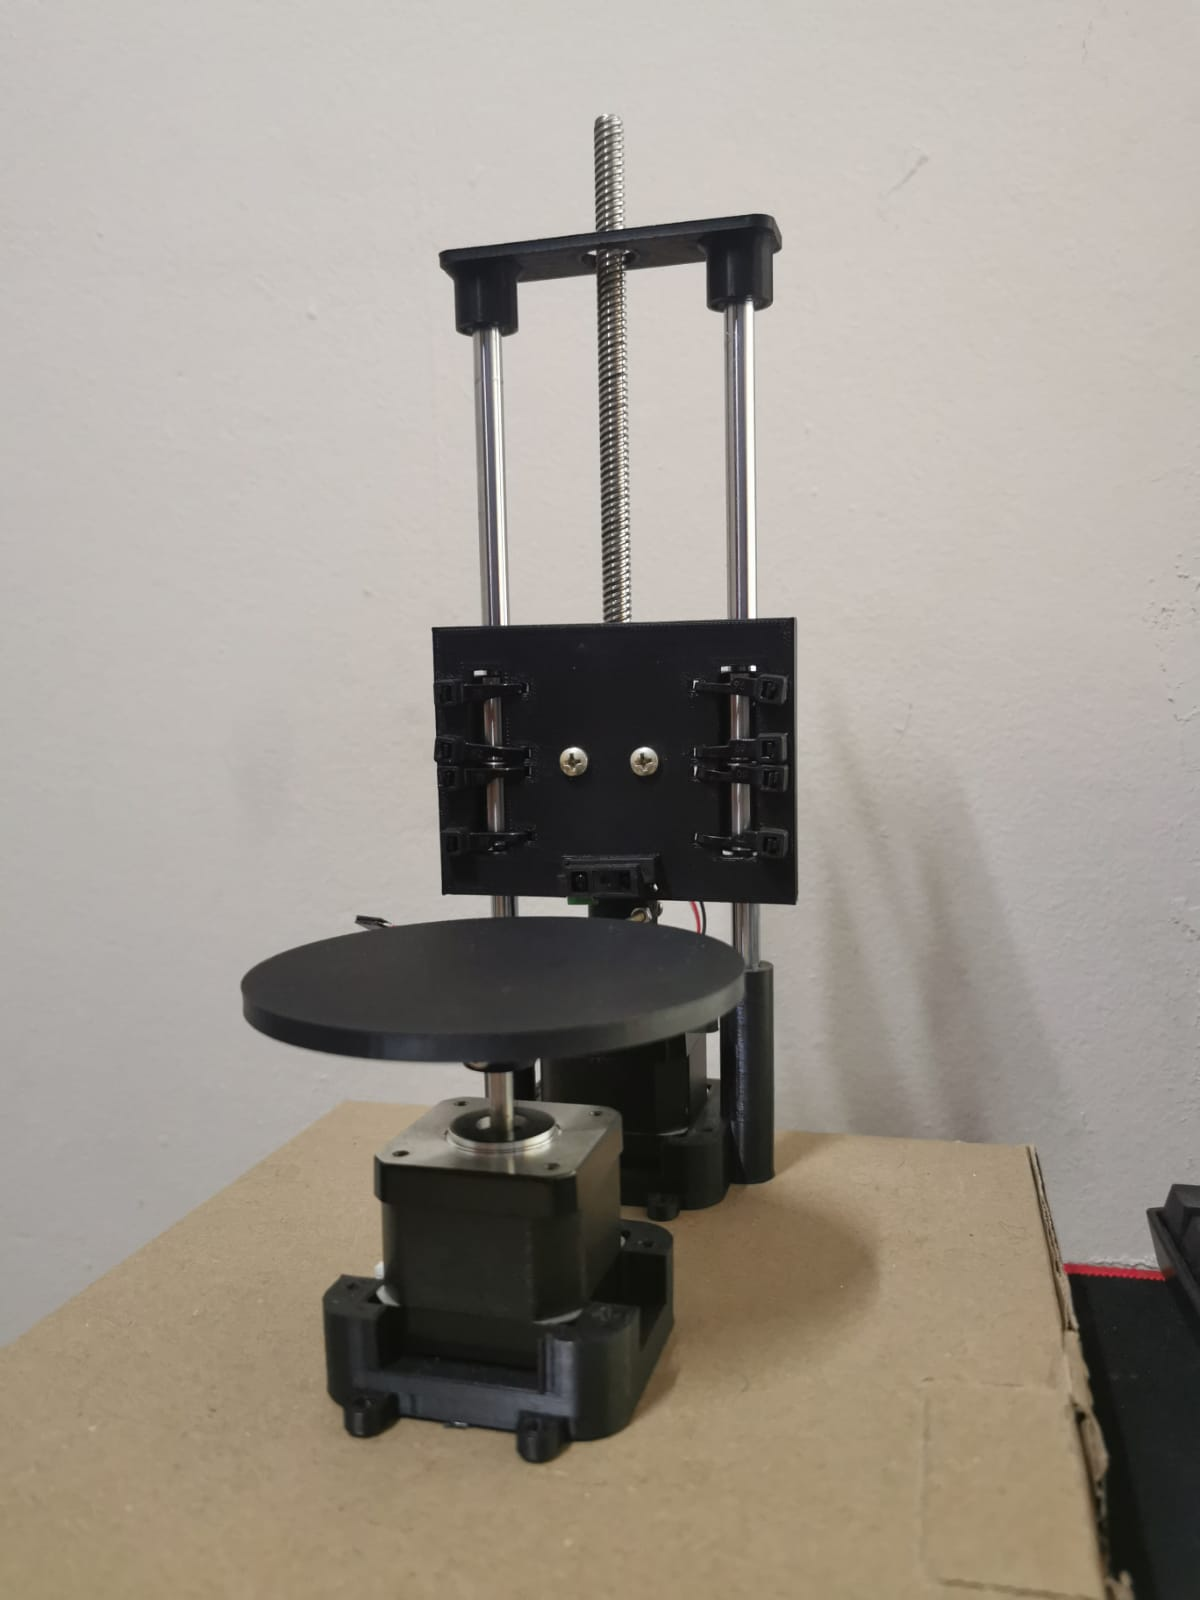
\includegraphics[width=0.45\textwidth]{3.Mecânica/Imagem/Estrutura.jpeg}%% Dimensões e localização
\fonte{AUTORES}%% Fonte
\end{figure}

\subsection{Bases dos Motores}

As bases dos motores são componentes cruciais na estrutura, responsáveis por fixar os motores de passo de maneira estável. São duas bases idênticas em suas dimensões principais, garantindo uniformidade na montagem e distribuição de forças. No entanto, uma delas possui características adicionais para acomodar os eixos.

Uma das bases é equipada com hastes verticais em forma de cilindros ocos. Estas hastes têm uma espessura maior, projetadas especificamente para comportar os eixos de 8mm de diâmetro. A inclusão dessas hastes permite um alinhamento preciso dos eixos. As hastes também adicionam rigidez à base, minimizando qualquer flexão ou deslocamento durante a operação.

\subsection{Fixador do Motor}

Ambas as bases, em conjunto com os motores, possuem fixadores superiores com encaixe para anexação dos parafusos que fixam longitudinalmente a base e o motor.

\subsection{Acoplador do Eixo}

O acoplador do eixo rosqueado faz a interface entre o eixo e o motor de passo, garantindo que a rotação de ambos esteja perfeitamente alinhada e sincronizada. Este acoplador evita qualquer deslize do eixo sobre o pino do motor, proporcionando uma transmissão de torque eficiente.

O design inclui um orifício central rosqueada internamente para se ajustar ao eixo de maneira segura e um orifício de encaixe no pino do motor, o mesmo possui um mecanismo de fixação, apertado por 2 parafusos para que o motor esteja firmemente preso ao acoplador.

\subsection{Plataforma do Sensor}

A plataforma do sensor foi projetada para segurar o sensor de forma segura e permitir seu movimento vertical preciso durante o processo de escaneamento. A mesma possui entradas específicas para parafusos e para a passagem de abraçadeiras de nylon que fixam os rolamentos por onde passam os eixos de 8mm.

A plataforma possui furos para permitir a fixação firme do sensor com parafusos, garantindo que o sensor permaneça estável durante o movimento vertical, evitando qualquer desvio que possa comprometer a precisão da captura das distâncias.

No centro da plataforma, há um ponto de fixação para um objeto rosqueado que se conecta ao eixo rosqueado principal. Esta conexão é crucial, pois permite que a plataforma se mova verticalmente conforme o eixo rosqueado gira, acionado pelo motor de passo. Este mecanismo é o que permite a elevação e descida do sensor durante o processo de escaneamento.

\subsection{Mesa Giratória}

A mesa giratória é a base onde o objeto a ser escaneado é colocado. Esta mesa é projetada para proporcionar um movimento circular controlado e preciso, essencial para a captura de todos os ângulos do objeto durante o processo de escaneamento. A fixação da mesa ao pino do motor é realizada através de um parafuso, permitindo um acoplamento mais firme.

A superfície da mesa é projetada como um disco plano e liso, proporcionando uma base estável para o objeto a ser escaneado. A dimensão dela foi calculada para acomodar uma ampla variedade de tamanhos de objetos pequenos e médios, garantindo versatilidade e precisão junto ao sensor.

A mesa possui um orifício central que se conecta diretamente ao pino do motor, ela possui uma passagem para o parafuso que fixa a mesa ao pino do motor de passo. Esta conexão garante que a mesa gire de maneira controlada e precisa em resposta aos comandos do motor.

\subsection{Guia Superior}

A guia superior foi projetada para manter os eixos em uma distância constante e fixa, garantindo a estabilidade e o alinhamento do sistema. Além disso, a guia superior possui um orifício central por onde passa o eixo rosqueado.

A guia possui dois suportes laterais projetados para segurar os eixos, mantendo-os na mesma distância entre si. Estes suportes garantem que os eixos permaneçam paralelos e estáveis, evitando qualquer desvio que possa comprometer a precisão do processo.

\section{Mecânica}

Abordaremos em detalhes os aspectos mecânicos do 3D Scan, incluindo os movimentos verticais e circulares essenciais para a operação do sistema. A sincronização desses movimentos é crucial para a captura das distâncias, e a mecânica envolvida desempenha um papel fundamental nesse processo. 

A seção está dividida em três subseções: o movimento vertical, o movimento circular da mesa e a sincronização desses dois movimentos para o escaneamento do objeto.

\subsection{Movimento Vertical}

O movimento vertical do 3D Scan é realizado pelo motor de passo que aciona um eixo rosqueado. A estrutura mecânica responsável por este movimento inclui a plataforma do sensor, o eixo rosqueado, os rolamentos, a guia superior e as bases dos motores.

\begin{itemize}
    \item A plataforma do sensor se move verticalmente ao longo dos eixos, guiada pelo eixo rosqueado.
    \item Conectado ao motor de passo através de um acoplador de eixo rosqueado, o eixo rosqueado transforma a rotação do motor em movimento linear vertical.
    \item Os rolamentos garantem um deslizamento ao longo dos eixos verticais.
    \item O guia Superior mantém os eixos na mesma distância e os fixa, assegurando a estabilidade estrutural durante o movimento. 
\end{itemize}

O motor de passo aciona o eixo rosqueado, convertendo a rotação em movimento linear. Conforme o eixo rosqueado gira, a plataforma do sensor, que está fixada ao eixo, se move verticalmente. Os rolamentos garantem que o movimento ao longo dos eixos seja suave e sem obstruções. A guia superior ajuda a manter os eixos paralelos e firmemente fixados, evitando qualquer oscilação ou desalinhamento.

\subsection{Movimento Circular da Mesa}

O movimento circular da mesa é gerado por outro motor de passo, que controla a rotação da mesa giratória onde o objeto a ser escaneado é fixado. A estrutura mecânica responsável por este movimento inclui a mesa giratória e a fixação ao pino do motor.

\begin{itemize}
    \item A mesa é fixada ao motor de passo através de um parafuso central.
    \item O pino do motor de passo se conecta à mesa giratória, garantindo que a rotação do motor seja transmitida de forma precisa à mesa.
\end{itemize}

O motor de passo aciona a mesa giratória, que é fixada ao pino do motor através de um parafuso. À medida que o motor gira, a mesa também gira, permitindo que o objeto colocado sobre ela seja rotacionado. Este movimento circular é crucial para capturar a distância de todos os ângulos do objeto durante o processo de escaneamento.

\subsection{Sincronização dos Movimentos}

A operação eficiente do 3D Scan depende da sincronização precisa entre o movimento vertical da plataforma do sensor e o movimento circular da mesa giratória. A combinação desses dois movimentos permite que o sensor capture uma série de distâncias de diferentes ângulos e alturas, resultando em uma digitalização completa e detalhada do objeto.

\begin{itemize}
    \item Início do Processo: O processo de escaneamento começa com o motor de passo vertical acionando o eixo rosqueado, movendo a plataforma do sensor para a posição inicial.
    \item Movimento Simultâneo: Conforme o sensor se move verticalmente, o motor de passo da mesa giratória começa a girar a mesa. A sincronização dos dois motores garante que o sensor capture distâncias a partir de diferentes alturas e ângulos.
    \item Precisão e Coordenação: A precisão dos motores de passo, juntamente com a estrutura, assegura que os movimentos sejam coordenados, evitando qualquer desvio que possa comprometer a qualidade do escaneamento.
\end{itemize}
